\chapter{Introduction}\label{chap:introduction}

Today's Internet

One example of such a scenario are
This results in a clash of interests which negatively impacts the network performance for all participants.

The goal of this monograph is
To this end, we study
If such an optimisation is not possible or attempts at it might lead to adverse effects, we discuss the reasons.

In the remainder of this chapter we first introduce the stakeholders considered in this work in \refsec{sec:introduction:considered_stakeholders}.
Then, in \refsec{sec:introduction:scientific_contribution}, we provide an overview over the scientific contributions of this monograph with respect to the stakeholders interest.
Finally, \refsec{sec:introduction:outline} provides an outline of this monograph.

\section{Scope of Considered Stakeholders}\label{sec:introduction:considered_stakeholders}


\section{Scientific Contribution}\label{sec:introduction:scientific_contribution}
This monograph studies the interactions between different stakeholders in three, partially overlapping, scenarios in order to provide an overview of today's interlocking network and application ecosystem.

\begin{figure}
\centering
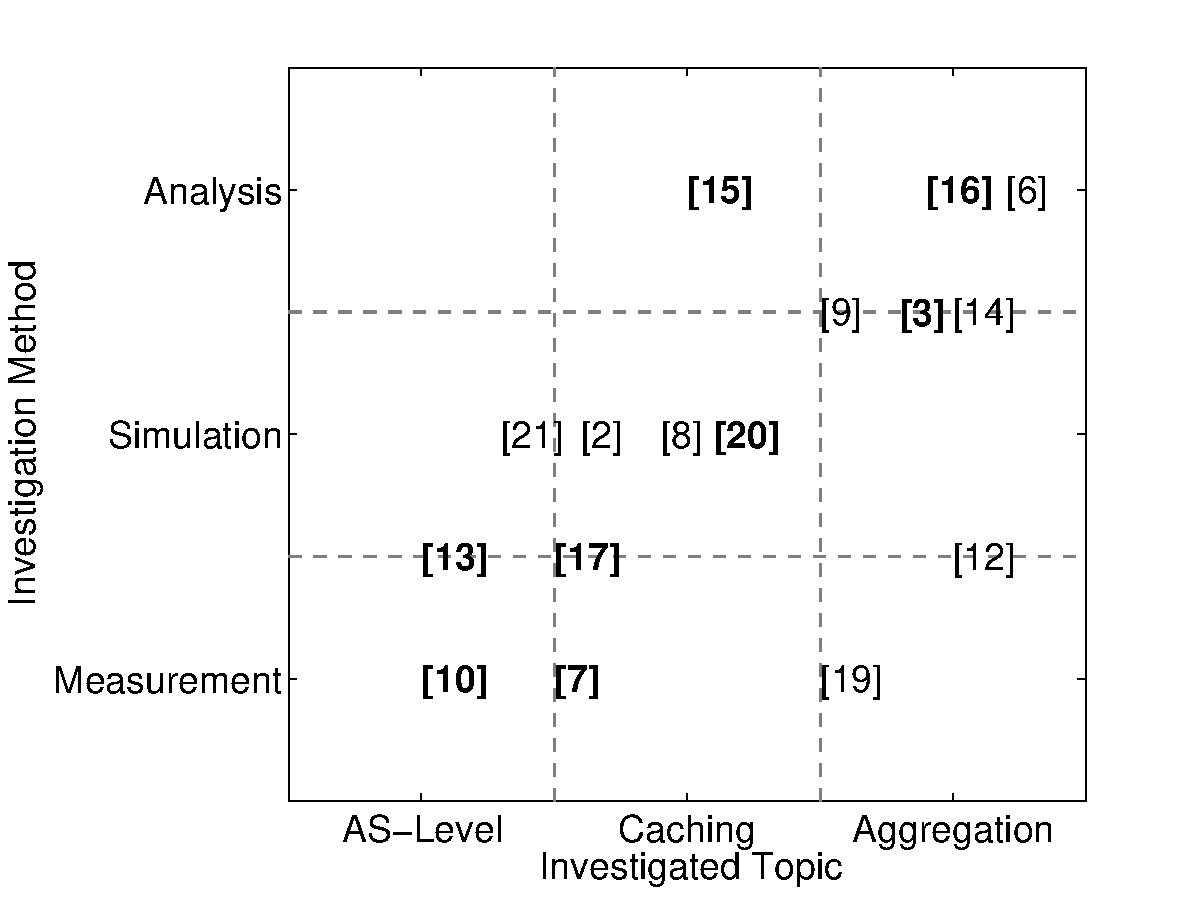
\includegraphics{figures/publications}
\caption{Contribution of this work as a classification of the research studies conducted by the author.}\label{fig:introduction:publications}
\end{figure}

In \reffig{fig:introduction:publications} we classify the areas of research as well as scientific methods used in relation to the chapters of this monograph.
The x-axis shows the impacted areas of research, i.e. topics related to the mobile network, the application domain or cloud technologies.
The y-axis details the applied scientific method.
In the theoretical area methods from queueing theory, mean value analysis and the analysis of random variables are used.
Measurements were performed using testbeds and custom software tools.
Simulation studies, performed using \gls{DES}, and created analysis tools are summarised in the practical area.

Annotations are used to highlight scientific publication whose content contributes to the respective chapters.

The first contribution of this monograph is a discussion of the impact of
We study the impact of , and investigate the potential of network parameter optimisation as a means to .

As a second contribution, we provide models for
We show that the streaming mechanism allows
However, further study shows that in fact
Furthermore, we provide

As a third contribution, we discuss the
To this end, we study the performance of
We derive guidelines for
Furthermore, we discuss a mechanism to
Finally, we present a mechanism to

\section{Outline of Thesis}\label{sec:introduction:outline}

In \refchap{chap:aslevel} we study
First,
Then,
Finally,

\refchap{chap:hierarchical} focusses on
For Video Streaming, we study the impact
To address the second scenario, we discuss

In \refchap{chap:aggregation} we study
First,
Then,
We analyse traffic characteristics and use them as input for a simulation model
Combining these results, we evaluate the impact of different virtual server configurations and scaling strategies.
Finally, we consider resource allocation

In \refchap{chap:conclusion} we provide a summary of the major contributions of this work and suggest future potential research directions.
